\documentclass{imc-inf}

\title{Data Mining in Sports}
\subtitle{Implementation and analysis of machine learning prediction models to find potential influential factors in results of matches in the Australian Football League}
\thesistype{Bachelor Thesis} % or Bachelor Expos\'e
\author{Thomas Gallagher}
\supervisor{Dr. Deepak Dhungana }
\copyrightyear{2023}
\submissiondate{02.04.2023}
\keywords {Data Analytics, Machine Learning, Sports Prediction, Neural Network}


\usepackage{listings}
\usepackage{subcaption}
\definecolor{codegreen}{rgb}{0,0.6,0}
\definecolor{codegray}{rgb}{0.5,0.5,0.5}
\definecolor{codepurple}{rgb}{0.58,0,0.82}
\definecolor{backcolour}{rgb}{0.95,0.95,0.92}

\lstdefinestyle{mystyle}{
	backgroundcolor=\color{backcolour},   
	commentstyle=\color{codegreen},
	keywordstyle=\color{magenta},
	numberstyle=\tiny\color{codegray},
	stringstyle=\color{codepurple},
	basicstyle=\ttfamily\footnotesize,
	breakatwhitespace=false,         
	breaklines=true,                 
	captionpos=b,                    
	keepspaces=true,                 
	numbers=left,                    
	numbersep=5pt,                  
	showspaces=false,                
	showstringspaces=false,
	showtabs=false,                  
	tabsize=2
}

\lstset{style=mystyle}


\begin{document}
	\frontmatter\maketitle{}
	
	
	\begin{declarations}\end{declarations}
	
	
	
	\begin{abstract}
		Despite the large amounts of data produced by the sporting industry every year, there has been relatively little crossover between academic data science and professional sports. On the other hand, Data Mining techniques such as Machine Learning, Neural Networks and Association Methods, have seen rapid increases in their complexity and use over a wide variety of fields and disciplines. 
		This paper aims to address this issue of a lack of data science applications in sports, with regards to the Australian Football League (AFL), by applying Data Mining techniques to improve upon already utilised data analysis techniques present in modern professional sports. In this paper statistics and results from the previous 10 AFL seasons will be assessed to identify key features and possible trends and use them to create more explainable white box prediction models. This will help not only sports professionals and data scientists but also casual viewers to understand the finer statistical details behind sports.
		
	\end{abstract}
	
	
	
	\addtoToC{Table of Contents}%
	\tableofcontents%
	\clearpage
	
	
	\addtoToC{List of Tables}%
	\listoftables
	
	
	%   MAIN MATTER  %%%%%%%%%%%%%%%%%%%%%%%%%%%%%%%%%%%%%%%%%%%%%%%%%%%%%%%%%%%%%%
	\mainmatter%
	
	\chapter{Introduction}\label{chap:introduction}
	
	This paper will apply Data Mining techniques on Australian Rules Football data in an attempt to identify any trends that may occur in individual seasons and then further apply this information into a Neural Network to create a prediction model for subsequent games.
	
	The field of Data Mining has seen a rapid increase as we enter the digital age dominated by digital information also commonly known as data. While many believe data mining to simply be the extraction of data it is actually a much broader topic. Data extraction is only the first step in data mining, the goal of data mining is to extract ‘previously unknown’ and unseen patterns from this data \cite{website:TechGuy}, much of which would be impossible to uncover without the help of computer systems. Data Mining is most commonly applied in commercial business. There it can be used to ‘help identify and predict individual and aggregate behaviour’ \cite{ACM}, or more commonly to predict how customers will consume/buy products and their buying habits so that they can more efficiently market their products in specific situations. Data Mining in sports however is much less advanced. Despite massive amounts of data being produced by the sporting industry, it is mainly kept behind closed doors, with much of its use being focused on player and team performance. It is also used to gain a competitive advantage over rivals clubs, which is the data is kept private.
	\newline
		
	Although it is a quite unrepresented research area, there have been some recent attempts at data mining in sports, which have been used in a variety of areas including, classification \cite{Displays}, action recognition \cite{AEJ} and image recognition \cite{Heliyon}. While data mining has also been used to aid in the creation of sports prediction models \cite{CollegeFootball}\cite{Basketball}\cite{LSTMPrediction}, none of these models aim to identify trends within the sports apply these as part of their prediction model. 
	
	An issue with many prediction models is the lack of transparency in their decision making, a key concept of this is issue is the idea of black box and white box models. Black Box models are in most cases more accurate than white box model but much more difficult to interpret, the internal decisions and processes of the algorithms are much more difficult to extract, resulting in more difficulty when wanting to view how they came to certain decisions. In this paper a combination of exploratory data analysis, data mining and feature extractions will be used in an attempt to overcome this lack of interpretability. Although the final prediction model will still be a black box model, the aforementioned methods will be utilised to extract meaningful interpretable information from the data set regarding which features are likely to have the greatest impact on the prediction model.
	\newline
	
	The final stage of the practical work will be to input the analysed data into a Neural Network to create a prediction model. Neural Networks are computing systems which aim to 'mimic the way that biological neurons signal to one another'\cite{website:IBM}. Neural Networks have a multitude of uses in a variety of fields including medical diagnosis by image classification, targeted marketing and financial predictions through behaviour data analysis and financial data processing, natural language processing and time series analysis. The use of neural networks in sports, like data mining, is very limited in the public domain. Unlike data mining the vast majority of neural networks used in sports deal with prediction models and cover a variety of sports codes. The most common applications are in Football (Soccer)\cite{website:Medium_Soccer}, American Football
	\cite{NN_NFL} \cite{CollegeFootball} and Basketball \cite{Basketball} \cite{Basketball_2}. 
	\newline
	
	In Australian Football, one of the most data rich sports \cite{website:Vice}, data is used in many ways. In a professional capacity this includes real time analysis of players and the modelling of games based on Geographical Positioning System (GPS). There also exist some prediction models created in both professional and non-professional settings, however in most cases the full data sets are only available in the professional environments. Most of the data and analysis models are kept internal and utilised only by clubs and a small group of media companies with rights to the data. As a result many prediction models rely on only a small subset of the collected data that is made available to the general public.
	\newline
	
	As this paper is discussing Australian Football a basic background should be given to understand some of the terms and structure of the game, as well as to understand the structure of the data set. 
	\begin{enumerate}
		\item On match day a team is made up of \textbf{22 players}, 18 on the field and 4 reserve players
		\item The aim is to score more points than the opponent by kicking the ball through either the \textbf{goals}, worth 6 points, or \textbf{behinds}, worth 1 point.
		\item Each team plays \textbf{22 games} per season, each season occurs between March and October in the Australian winter.
		\item The finals are contested between the top 8 teams from the regular season, the finals series lasts for \textbf{4 weeks}
		\item There are currently \textbf{18 teams} in the competition.
		\item 10 teams are based in Victoria. New South Wales, Queensland, South Australia and Western Australia each have 2 teams in the competition.
	\end{enumerate}
	
	This paper aims to explore the impacts of external factors on the outcomes of Australian Football matches and generate interpretable results which can be utilised in further analysis and prediction of matches.
	
	
	\chapter{Background}\label{chap:background}
	\subsection{Research Questions}
	
	The area of focus of the paper is the implementation and analysis of machine learning models to find potential influential factors in results of matches in the Australian Football League (AFL).
	From here I have defined the following research questions which will be explored:
	\begin{enumerate}
		
		\item[] Can data mining be used to find key features and explain results in professional sports?
		
		\item[]Can these extracted trends and features be used to create an reliable prediction model?
		
		\item[] How effectively can Long Short Term Memory neural networks be used to predict sports outcomes?
		
		\item[] If the model can reliably predict outcomes, how many rounds will the model need before it becomes reliable?
	\end{enumerate}
	
	
	\subsection{Technical Background}
	The practical section of the paper will follow a basic flow of a Machine Learning process (ML Process) for a classification problem. Which follows the format of Problem Exploration, Data Engineering, Model Engineering, Deployment and Monitoring. Data and Model engineering will be the main areas of the data flow applied in the practical section.
	
	Classification is a technique in which the model tries to predict the discrete class of a given input data. This is also a supervised problem meaning that the classes are already known to the model and as such no additional methods will be needed to extract the classes from the data set.
	\newline
	
	The data engineering phase deals with the acquisition, cleaning and exploration of the data set. Data engineering is a very important part of the ML process, as it is critical to have clean and consistent data for a model to function correctly. Without clean data a model cannot be trained efficiently, the model will be unable to extract any meaningful information from the data. 
	\newline
	
	The data acquisition process can vary between projects. In the simplest cases, a data set can be readily and publicly available, needing only to be downloaded before the cleaning and exploration phases can take place. With more complex or industry specific data sets, the data may already exist but be owned by an institution which measured, converted and stored the data set. In these cases the data is normally available via payments or contracts. In the most complex cases the digital data set does not exist at all and must be gathered from physical real-world data and converted into a digital data set by the members working on the project. 
	\newline
	
	Once the data has been acquired Exploratory Data Analysis (EDA) can be performed. EDA is the initial analysis of the data set, it allows for a basic overview of the characteristics of the data to be investigated and identified. Additionally EDA can allow for the easier detection of anomalies and errors within the data set which can be handled in the data cleaning phase. The main method of EDA is data visualisation, which allows for the entire data set or individual features to be viewed in plots. Correlation analysis and histograms will be utilised in the paper in the initial analysis of the data.  Correlation measures the relationship between variables, and generally a value between 1 and -1 is given to describe this relationship. A correlation of 1 means the values share a positive relationship, an increase in one of the values leads to an increase in the other, while -1 is the opposite an increase in one leads to a decrease in the other. Additionally a correlation of 0 means that the two values are independent and have no relationship with each other. Histograms are used to separate quantitative values into an interval scale, these interval groups can be used to identify where distributions lie within the data set. In addition a basic description of the data set will be analysed, pandas dataframes offer functions to describe the contained data in each column, which will be used to view the averages, standard deviation and percentile distributions of each column in the data set.
	\newline
	
	Data cleaning ensures that the incoming data is able to be read and interpreted properly by the computer model. The important steps are ensuring that missing values are handled gracefully, either by removing affected rows and columns, or using imputation to replace null values.
	The data must also be formatted correctly so that it can be read by the model. As the data is being read by a machine this is in most cases a numerical input. In this paper two methods will be used to convert text and categorical inputs to numerical values, integer encoding and one hot encoding. Integer encoding involves converting every unique categorical value to a numerical value and replacing the original value in the data set. The issue with integer encoding is that models can also infer false information from the values, one way this occurs is that the model can assume the categorical values have a specific order that applies to them inferred from the order of the numerically encoded values. The solution to these issues is to use One Hot Encoding, this is when a binary value is included for each categorical value. This separates each value into its own feature that the model will interpret individually.
	\newline
	
	The final phase of the Data Engineering is the feature engineering process. This is the process of extracting features from the raw data set which can be used by the machine learning model to enable it to understand the data. In the case of tabular data, as is being analysed in the paper, a feature is one column of the data. Feature Engineering generally consists of four processes "Feature creation, transformations, Feature extraction and Feature selection" \cite{website:JavaTPoint}. Feature creation is the creation of features based on domain knowledge and human input or intuition. Transformations deal more with the adjusting of the data to ensure that all of the data is in a similar scale, this can be done via normalisation which converts every value in the data set to a value usually between 0 and 1, or -1 and 1. Min-max normalisation $x' = (x - min) / (max - min)$, is applied to each feature in the data set and normalises the feature values between 0.0 and 1.0 based on the minimum and maximum value present in each feature. Feature extraction "generates new variables by extracting them from the raw data" \cite{website:JavaTPoint} via detection algorithms, these are also used to combine and reduce the number of variables used in the final model. This will not be utilised in the paper due to the available data set already containing a limited number of features. The final stage is the feature selection, after all of the features have been established, the features that are most useful for the end model in its predictions are identified, and the remaining irrelevant features which  have no impact or a negative impact on the results of the model are filtered out from the data set. 
	
	Data set splitting also occurs during the data engineering phase. The data set needs to be split into a training set which will be used to train and tune the model and a testing set which will be completely held out from the training phase and used to analyse the final model on unseen data. Additionally a validation set can be created to aid in the training phase, similar to the testing data set, the validation data is also held out when training the model, but is used to analyse the model during the training and tuning phase. Commonly between 70 percent and 80 percent of the data is used for the training set, with the rest being evenly split between the validation and test sets. 
	
	Decision Trees and Random Forests are extremely useful prediction tools, as they can also be used as feature extraction tools. Decision Trees are a "supervised learning method used for classification and regression" \cite{website:SciKitTrees}. Supervised learning is a machine learning method in which the model is presented with both input and output data so that it can learn the relation between the two and predict the outputs of new input data. The aim of a Decision Tree in classification is to split the data set into subsets called nodes until each node contains only data points of the same class, sometimes called pure leaf nodes. At each node a decision is made by the model which attempts to create a node that is as pure as possible, there are many ways to test for the purity two of the most common are the gini index and entropy. The Gini Index "measures how often a randomly chosen attribute it misclassified", whereas Entropy "measures the impurity of the sample values" \cite{website:IBM_Trees}. 
	\begin{equation}
	GiniIndex = 1-\sum_{j}p_{j}^{2}
	\end{equation}
	\begin{equation}
	Entropy = -\sum_{j}p_{j}\cdot \log_{2}\cdot p_{j}
	\end{equation}
 	Both methods are quite similar and have the same aim to minimise the function, have a value as close to 0 as possible.
 	Where Decision Trees become useful in feature engineering is they store the decisions they made and from this can later compute which features had the greatest overall impact in the model. 
 	While Decision Trees are useful, they do tend to overfit to the training input data, they become very good at predicting the training data but do not perform as well when introduced to new unseen input data. There are multiple ways to penalise a decision tree, to stop it from over fitting to the training data. 
 	Setting a depth level will ensure that the tree will only make a predefined number of splits before stopping. If this is not set the tree will continue to grow until every leaf node is pure, meaning the splits will be too specific to the input data. With a limited number of splits only the more general decisions will be found, which should then be able to explain new unknown data. 
 
	A minimum node size can also be set, this stopping criteria will stop the model from splitting a node further once the subset of data in the node reaches a minimum size. A larger minimum node size will result in a smaller tree being made and as such will prevent the model from overfitting to the training data. 
	
	It is also important not to set the stopping criteria too far in the opposite direction and reducing the complexity too much. This would result in the model underfitting and not being able ascertain any valuable information from the data. 
 	\newline
 	
 	Random Forest is an extension of Decision Tree methods that utilises multiple Decision Trees to reach a prediction. Random Forests consist of a collection of Decision Trees that are each trained on a different random subset of the original data set. A random forest has multiple hyper parameters that must be set before training, these include node size, number of trees and number of features to train on. The Random Forest model will create the specified number of trees and then for each tree it will select the random selection of the data set, and then it will randomly select the features based on the number of features defined in the hyper parameters. All of the trees will then be trained on their individual data sets and the results of all the trees will be used to decide on the final result and the most important features present in the data.
 	\newline
 	
 	For many ML projects using Decision Trees or Random Forests will cover both the feature engineering and the Model Engineering phases. Other models can still be built in the model engineering phase, with the Decision Trees acting as not only a feature engineering tool but also a comparison tool for the final model. In this paper a more complex neural network will be built to further analyse the data in the model engineering phase.
 	
 	Neural Networks are computer systems designed to replicate the neuron systems in biological brains. They consist of a collection of nodes, also called perceptrons, organised in layers that mimic the way that biological neurons communicate. 
 	There are three distinct types of layers in Neural Networks, each contains one input layer, multiple hidden layers and one output layer. All of the nodes are interconnected between layers. Each node takes the input data, either from previous layers or from the input data, and analyses it in a fashion similar to multiple linear regression. The formula for a Neural Network perceptron is shown in figure 2.1. Once the inputs have been computed by the formula the results are passed through an activation function which decides whether the neuron is important and if it should be activated or not. The activation functions also remove the linearity from a neural network. As the basic formula of the neural network follows the linear regression formula, the outputs would also be linear. By using the activation functions to add non linearity to the outputs it allows the Neural networks to find more complex representations of the input data. 
 	\begin{equation}
 		Linear Regression: y = b_{0} + b_{1}*x_{1}
 	\end{equation}
		\begin{equation}
		Multiple Linear Regression: y = b_{0} + b_{1}*x_{1} + b_-{2}*x_{2} + ... + b_{n}*x_{n}
	\end{equation}
	\begin{figure}
		\caption{Basic Neural Network Formula}
		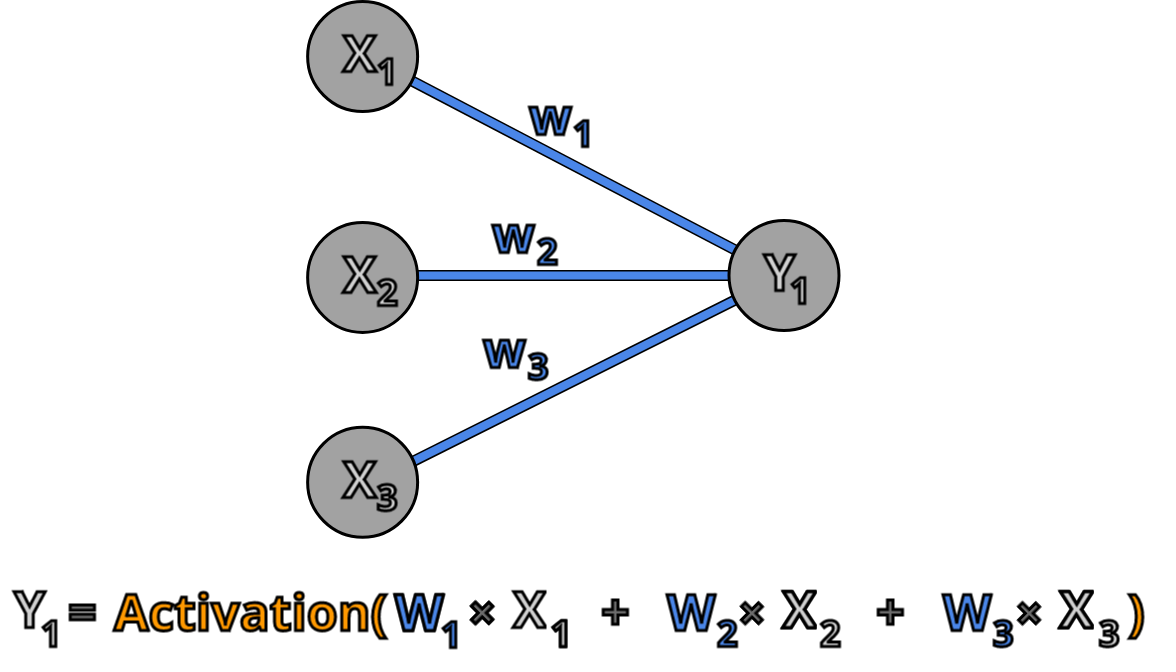
\includegraphics[width=10cm]{media/nn_formula.png}
		\cite{website:BH_AI}
	\end{figure}
	\newline
	There are two commonly used activation functions in neural networks, sigmoid and tanh. Both functions are quite similar in that they limit the input to within a certain range, the sigmoid function returns a value in range of 0 and 1 whereas tanh returns a value in range of -1 and 1. \cite{website:Activation}.
	
	\begin{equation}
		Sigmoid: s(x) = \frac{1}{1 + e^{-x}}
	\end{equation}
	\begin{equation}
		Tanh: tanh(x) = \frac{e^{x}-e^{-x}}{e^{x}+e^{-x}} = 2s(2x) - 1
	\end{equation}
	
	
	Traditional Neural Networks also face an issue of handling sequential data, which is partly solved with Recurrent Neural Networks (RNN). RNN add a memory element to traditional Neural Networks, meaning that the output of the previous layers are remembered sequentially. The most common applications of RNN are within time series forecasting and natural language processing. The issue with RNN is that "they cannot learn long term dependencies due to vanishing gradients" \cite{website:AV_LSTM}, this occurs because the weights of the previous layers that are passed through each stage are multiplied which will always result in a smaller number, meaning the loss will decrease towards 0. Long Short Term Memory networks (LSTM) overcome this issue by introducing memory gates (Figure 2.2).
	\begin{figure}
		\caption{Long Short Term Memory network gates}
		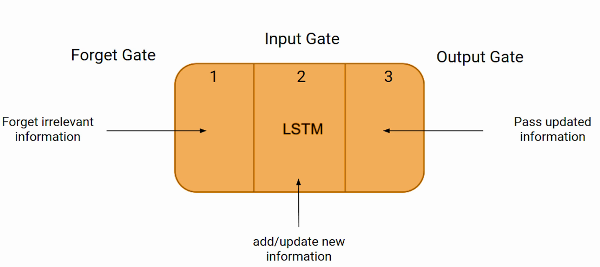
\includegraphics[width=15cm]{media/LSTM.png}
		\cite{website:AV_LSTM}
	\end{figure}
	The forget gate analyses the information from the previous time step, called the hidden state and decides whether it is important and should be kept of if it should be forgotten.
	The input gate is used to identify the importance of the current input values.
	The output gate determines the value of the hidden state which will be stored and analysed in the next time step.
	\newline
	
	After the model has been built and tuned to produce the best result, the Deployment and Monitoring phase can begin. 
	
	The first section of this paper will be the exploration of the data set with the aim of identifying trends and important features within the data. Important features are features that have a greater impact on the final result of a prediction model. Trends will be defined as features or feature patterns that occur in multiple seasons. Both known and unknown features and trends will be extracted and from the data set. Known features will be defined as factors that are currently used in analysis of sports games, which stem from less scientific analysis of data. These known features are generally used in predictions of games by both domain experts and casual observers and are widely accepted to be true, but there has been little research to provide evidence to the claims. The unknown features and trends will be discovered during the data exploration and will be represented by the important features, the factors which have the greatest effect on the outcome of the model, extracted during the feature engineering process.\newline
		
	In the analysis of AFL games there are many factors that are said to have an impact on results by domain experts and casual viewers alike, these factors will be analysed as known features in the data set. There are two main ideas behind exploring these features. Firstly, it is useful to take domain knowledge from experts, even if it second hand as in this case. Having access to expert domain knowledge can provide a solid foundation in data analysis workflows, it allows for the analysis to be applied in a specific area of the data set without the need for pre-analysis and feature extraction. The second reason is to statistically analyse whether there is any truth to these claims and if this analysis can be useful when used as a feature in a computer aided prediction model.
	\newline 
	
	The main points that will be explored from this expert analysis are the effects of weather conditions both during and in subsequent games, the length between games and the impacts of travel on future results. The impact of weather will be analysed in two features, the first being the impact of a previous games rainfall conditions as it is believed that it can negatively affect a team’s performance in future weeks, as the game becomes more contested thus requiring a greater physical output. The second will be the impact of rainfall on a current game, rainfall during games generally reduces disposal efficiency making results closer, and also different game plans are impacted more by rainfall thus it can be assumed that rainfall will have some correlation to specific teams (rainfall for the model will be taken as predicted rainfall, connected to teams). While with travel it is suggested that spending long times in planes both before and after games can affect a teams’ recovery and preparations. There has been research done on the impact of weather on team performance in the AFL\cite{website:AFL_Weather}, which focuses on the analysis of results as such the findings are not used to aid in any prediction models, which this paper aims to do.
	\newline
	
	While trends can be extremely useful for prediction they can also be difficult to interpret and extract from data. This is another reason why the expert analysis is being explored. It gives a starting point from which the data can be analysed. Basic visualisation of the data set will be used to asses the expert analysis. Further extraction of trends will be entirely theoretical and based solely on algorithmic interpretation of the data set. This will be very important for the project as it will hopefully enable hidden features to be found, rather than just proving or disproving already voiced opinions. These trends would be much more valuable in the industry as they would give professionals a completely new insight into their analytics.
	
	The final key section will be the implementation of a prediction model. Prediction models are used regularly in sports. However as there are so many unknown factors in these prediction models it is very difficult to explain their predictions and how they came to these decisions. The aim is to create a prediction model based on the extracted trends and important features, that is more explainable than other models. 
	Assuming that the prediction model does reliably work, one more key piece of information will be extracted, the final research question, what number of rounds/games does the model need before it can reliably predict the outcomes of games? This can be useful not only for this model but for other prediction models for the AFL, as it can give a greater understanding of when results and match data will stabilise and become reliable in defining the characteristics of a season. The general consensus is that after 4 - 6 weeks of matches is when a reliable data set begins to form.
	There are many algorithms and techniques that can be used in Data Mining and sports, this paper will mainly utilise the following:
	
	\begin{enumerate}
		\item[] Decision Trees: A tree like predictive models that shows where certain decisions were made via nodes.
		\item[] Random Forest: A collection of decision trees, that uses a random subset of the data in each iteration.
		\item[] Long Term Short Term Neural Networks (LSTM): A type Neural Network that introduces the concept of memory and feedback connections allowing it to process data sequences.
	\end{enumerate}
	

	
	\chapter{Method}\label{chap:method}
	\section{Description of the Scientific Method }
	
	\subsection{Technical Environment}
	The project was completed using python as the main programming language, a combination of Jupyter Notebooks and Python files were created to handle different tasks. Jupyter Notebooks were used to sequentially implement workflows of the project and define minor functions. Major functions and more complex code were written in Python files which were accessed in the necessary code blocks within the Jupyter notebooks. There was no traditional database structures used, the data was stored in csv files. 
	There were many libraries used over the different stages of the implementation, in depth explanations of their uses will be given in the individual phases. The pandas library was used throughout the entire project as the main data handling tool. All data was accessed using pandas read csv functions to store the data in Data Frames within the project and the to csv function was used to store the manipulated data sets.
	Numpy was used for additional data manipulation in combination with pandas.  
	The Selenium library was used in the data acquisition phase to scrape additional data which was not available in the original data set.
	Scikitlearn, a machine learning library for python, was used in the implementation of the feature engineering and prediction models
	Treeinterpreter library was used in feature engineering to analyse the Decision Tree and Random Forest models.
	Tensorflow and Keras were used in the prediction phase to build the prediction models.
	
	The code used for this thesis can be found at:  \url{https://github.com/TomGallagher98/Thomas_Gallagher_Thesis}
	
	\subsection{Phase 1: Data Acquisition}
	The main dataset was taken from Kaggle \cite{stone}. It is a comprehensive dataset, containing statistics from every AFL game between 2012 and 2021 and is comprised of 3 tables. Games, containing data about the games and environment of the games, it contains 12 columns. Players which contains player basic information in 7 columns. Stats containing individual player statistics for every game has 31 columns. Overall there are over 90000 data points across the three tables.
	
	However there were some values that were not present in the original data set, which were required to enhance the data. The data set did not contain any values that rated player performance, which is a useful data point in sports prediction models. There are two prominent player scoring systems in the AFL, "Supercoach" and "Fantasy", which comprehensively rank every player after each game. To acquire this data I utilised scraping software selenium to scrape and store both sets of player scores from footywire.com. 
	
	Additionally some values needed to be manually calculated from the raw data set, these were all handled in the feature engineering phase to construct the final data set.
	
	\subsection{Phase 2: Data Engineering}
	Data Engineering is a key process in any data science project. Without good clean data it is nearly impossible to generate clean useful results from a model. 
	At the end of the data acquisition phase I was left with a data set that required considerable cleaning. The acquired data was stored in 4 sets, 'Games', 'Stats', 'Fantasy' and 'Supercoach'. The Players data set identified in the acquisition, only contained basic meta information about the players to it was left out from project. I also decided that the data should be split into individual seasons, firstly to reduce the computation needed to analyse the data final data sets, and also to allow for the analysis of each individual season. The main data engineering was thus divided into three stages, split each data set by year, for each year merge required features into central data set, from here the data could be analysed with basic exploratory data analysis (EDA). The merging of the data set overlaps slightly with the feature engineering as I was only choosing a selected set of data to merge into the final data set. But this was necessary to be able to perform any sort of initial analysis on the data, having the data spread out in different data sets would not yield as insightful results during EDA. Every feature was calculated for the home and away team separately, to avoid repetition when I will discuss the features as a group and not distinguish between the home and away feature.
	
	Splitting the data set by year was the simplest of the phases. Each csv was read into python as a pandas data frame. From there a script was created to separate each data set by year and create individual data frames for each year, these were then saved into individual csv files.
	
	The largest section of the data engineering was the merging of the data sets into one central group of data. The idea was to build the data around the 'Games' data set, because this already contained the results information from which the final model would be building the prediction. No columns were removed from the data set until the data was being fed into the final model. This was to keep the data set as complete as possible, in case extra features needed to be computed from the existing data then there would be no missing data which would need to be re-acquired. 
	
	To identify the team changes and previous results I created a python script entitled team changes. This which counted the number of changes between the selected team and the team the previous week.

	The distance travelled by each team was also calculated. Travel can be hard to define so it was calculated based on the teams home location. Each group had up to 6 travel categories based off the distance between their home location and the location of the game. 
	
	Ladder positions were taken based off two factors. The first was the historic ladder, so that the model could view where the team had finished in the previous season. For the historic ladder I decided to hard code the final positions and then create a data frame to match each team to the ladder position. This was then used to create the LadderPosition columns. The CurrentLadderPositions required a ladder model to be created. I generated this by creating a set of data frames for each round in the season, they tracked the teams, the points score by the team, the points scored against the team, the teams percentage (points for / points against * 100), and the total points (win = 4, draw = 2, loss = 0). To fill in the data each round was iterated over and each corresponding field was updated, the ladders were then ordered by points and percentage. Once the set was created the fields were added to the main data structure, along with each teams total points for, points against and percentage.
		
	The Fantasy and Supercoach data is used to give an overview of the strength of each team based on the players in the selected sides. I had the option to either include each individual player in the final data set, or to combine the scores from every player and only include this value. I decided on the latter option, as it allowed for the result to stay consistent in its position in the final data set. If I were to include individual player scores as features, it would have required either a column for each individual player, or 22 columns for all selected players but the order of the players would not be consistent. I believed it would be better to have one consistent overall value to describe the teams as opposed to the more inconsistent and changing values.
	
	As the main data set and the supercoach and fantasy data sets were acquired from different sources they required the greatest level of preparation to be able to merge the data sets. The naming conventions between the data sets were slightly different, both player names and team names varied between the data sets. This became an issue when attempting to extract values from the supercoach and fantasy data sets, as I was using these names to search for the corresponding data. The first step taken was to find the inconsistencies in the player names as this was a more difficult process. First I created a script to identify which names were present in either of the data sets that were not present in the other. From here I could view which names were different and which naming conventions were different. After multiple iterations I had discovered and removed the major inconsistencies and was left with only a handful of differing names, in this case I hard coded the name in which I wanted to keep as there were so few names left that it was the quickest option. The same process needed to be repeated for the team names. This was a much quicker process as there were only 18 names to analyse in each data set, meaning I could easily hard code the changes I needed and update the supercoach and fantasy data sets.
	
	The fantasy and supercoach points combined for each player to give an average value between the two as they performed the same function of rating the players, the entire teams average was then used in the final data in 4 features. TeamImportanceDifference, marked the average scores of players who played in the previous match but were not selected in the forthcoming game. TeamImportanceLastGame, calculated the average score of the team in the previous game. TeamImportanceLastFiveGames, calculated the teams average scores over the previous five games to asses a teams recent form line, if 5 games had not been played then the average was taken from the games that had been played. TeamImportanceSeasonAverage, calculated the average over the whole season for the team.
	
	The final data points added were the break between games for each team. This was done with a simple python script to find the number of days between the previous game that the team played and the upcoming game. To simplify the script it initially only looked at games from the previous round, this needed to be updated to consider games from the previous two rounds because bye rounds resulted in no games being identified in many cases. The break was initialised to 7 days as this was the median value identified. 
	
	The final stage of the data preparation was one hot encoding of team and venue data. One Hot Encoding (OHE) is a way to add categorical data into computer models that require a numerical input. Each venue and team are assigned a numerical value which is then added to the data set in place of the text value. In some cases the model will incorrectly assume that the size of the numerical numbers is an important factor, to combat this each category is assigned as its own feature in the data set that is either active (1) or inactive (0). This was only implemented in the final stages of the model and not added to the main data set, because some functions in the EDA and feature engineering sections perform better without OHE as it also creates a large number of empty variables in the data set.
	
	Once the main data set was built EDA was then used to explore relationships within the data. This was mainly implemented on features that had been proposed by domain experts. The main method used in the EDA was correlation analysis. Pandas Dataframe objects have a built in correlation function to generate a correlation matrix for every feature in the data set. This was then reduced to extract only the correlation of each value to the output variable 'homeWin'. Additionally a simple histogram was created to show the distribution of the homeWin feature. 
	
	\subsection{Phase 3: Feature Engineering}
	Once the final data set had been defined in the data engineering phase, the data was then analysed in the feature engineering phase. The models used for feature engineering were decision trees and random forests. Although the models are traditionally used for prediction and classification, they can also be used in feature engineering as they are able to track which features were most important when creating a decision node, which can then be analysed for the final model. Also as they do provide a prediction model it allowed me to have extra prediction models to compare with the final results of the project. 
	
	Before the data could be inputted into the model it needed to go through a final phase of pre processing. The y value, which was taken as the home team winning, was first separated from the data set. Two sets of y values were analysed. The first set analysed wins, losses and draws, the second set simplified this to only win and loss. Draws only made up 1 percent of total game outcomes, resulting in a significantly underpopulated feature, which could dramatically affect the result of the model. I didn't want to use any upsampling, creation of extra data rows, as I wanted the data to be as close to real life as possible. So to overcome this problem I decided to perform the feature engineering with both sets of y values.
	
	Label encoding was used to remove the text values from the data set and replace them with numeric variables. One Hot Encoding was not utilised during feature engineering, due to the smaller number of variables and the number of features that required OHE being quite large this would have created too many empty data points relative to the size of the data set. After the encoding all unused variables were dropped from the data set, these points comprised of metadata about the games (date, gameID, year, round, startTime), values that had been encoded (teams, venue) and features that described the outcome of the games (homeWin, homeTeamScore, awayTeamScore). Normalisation was then applied to the data set. This was done using a MinMaxScaler which reduces the size of the data points but keeps the original scale of each point. A min max scaler computes the points distance from the minimum value in the feature and divides it by the total range of the data in the feature, this reduced the range of the data points between 0 and 1.
	
	\begin{equation}
		Min Max Scaling: X_{std} = (X - X_{min}) / (X_{max} - X_{min}))
	\end{equation}
	
	Once the data had been normalised it was returned as a numpy array however I needed to transform it back into a pandas DataFrame to be able to view the columns in the final stages of the feature engineering. The normalisation steps were repeated however an extra step was added to extract the columns from the initial DataFrame, then once the normalisation was applied the data was transformed back into a DataFrame keeping the stored columns of the original data set.
	The data set was both split by year so that each season could be analysed individually, and joined into one single data set so that the model could analyse the entire volume of data. This resulted in 11 separate data sets which would be analysed. The train test split was set to .8 : .2, for the year by year data the model was trained on the first 19 rounds and tested on the final 4 round. The only exception being the 2020 season which was shortened due to COVID, the final 4 rounds were still held out for testing leaving only 14 rounds to train the model on. The merged data set was trained on the first nine seasons with the final 2021 season held out for testing. A baseline score was also identified for each data set to determine the percentage of homeWins per season so that any future predictions could be analysed in relation to the baseline. 
	\newline
	
	Before the features could be extracted the models needed to be trained and have the hyper parameters tuned to ensure the features were extracted from the best performing models. The first model created was a basic decision tree classifier (DT). The DT was also to be used as a baseline prediction parameter. Instead of being used to describe the ground truth the DT would be used to describe the prediction capabilities of a basic model on the data set. As such no hyper parameter tuning was performed on the DT. The model was first trained by fitting the training X and y values on the DT. Then a score was generated to display the average accuracy of the model on the validation data. Finally a prediction was made using the 'predict' function, a function print score was also defined to display the confusion matrix of this predicted outcome against the true  outcome of each game. 
	\newline
	
	Once the DT models had been established a Random Forest Model (RF) was created for each data set. The RF models are the main models used in the feature engineering so there were 3 phases of tuning on each model to extract the most important features.
	The first RF models were also quite basic, they consisted of 200 trees, and all of the default parameters of the scikitlearn RandomForestClassifier model. 
	The second RF models a grid search was used to establish the best hyper parameters for the model. The grid search was implemented on each data set and was populated with the following criterion: 
	\begin{center}
	\begin{tabular}{c c}
		'criterion': &['entropy','gini'] \\
		'min samples split': & [3, 5, 7, 9, 10] \\
		'min samples leaf': & [8, 9, 10, 11, 12] \\
		'max features': & [0.5, "sqrt", "log2", 0.8] \\
 		'n estimators': & [50, 100, 200]
	\end{tabular}
	\end{center}
	
	The best estimators were then extracted from the second RF model to create the third RF model. The third models were trained and fitted on the data sets as in the previous steps. To extract the feature importance the treeinterpreter python module was used. A script from fast ai was used to extract the important features from a RF model given an inputted data set in this case the x values of the problem set, returning a pandas DataFrame of each feature and its importance score. The data frames were then plotted to visually analyse the distribution and scale of the important features over each year. The top 20 features were then extracted from each model, a weight of 20 was given to the most important feature extracted and 1 was given to the least important feature, these were then tallied to identify which features were the most important over all years. As the majority of features were paired between home and away teams, if only one of the features were present the corresponding feature was also included in the final feature set, replacing the lowest ranked features. After this process the top 20 features selected for the final feature set were: 
	\newline
	
	The final stage of the feature engineering was to run a final RF model on the data set containing the selected features to identify one last base prediction to have in comparison to the final prediction model. The final RF model used the same hyper parameters utilised in the third model and the data set was reduced from the original data set to only include the important feature set.
	The final confusion matrices were then plotted to view the performance of each model.
		
	\subsection{Phase 4: Predictive Model}
	The final phase was the constructing of the prediction model. The prediction model used was a Long Short Term Memory Neural Network (LSTM), the LSTM models were implemented using the keras python library. Again only the final pre processing steps needed to be taken. The original data set was again imported from the csv files separated by year. The string values of the data set then were both label encoded and one hot encoded. This differed slightly to the feature engineering steps, in which the data was only label encoded. This was due to decision tree based models such as random forests performing worse on the sparse data distributions created by one hot coding, while Neural Network models are generally not negatively impacted by OHE. I also did not want the model to infer any immediate relationship between the team and venue data sets, which is a common issue when only applying label encoding. 
	\newline
	
	After encoding the labels the unused features were dropped from the data set. Two different data sets were created in this step. For the main data set only the features identified in the feature engineering were kept in the final data set, along with the OHE team and venue features. Although the two feature sets were analysed in the feature engineering phase as label encoded values and as such were subject to the same ranking principles applied in the the feature engineering phase, I decided that as they were two key features in general sport predictions they should not be removed, also OHE these features meant that different weights and importance could be determined for the features compared to the label encoded features which were in the feature engineering data set. The second data set comprised of the entire data set used in the feature engineering. This was done to asses the impact of the feature engineering and selected features on the final model, it would provide an insight on whether the RF model and final model extracted similar implications from the data set or whether the LSTM was able to understand the full data set better than the reduced data. As LSTM models are generally used for time series data, the order of the data sequence is an important factor, so the data set was not shuffled for when inputted in the final model.  	
	\newline
	
	The splitting of the data set followed a similar pattern to that which was used in the data engineering phase, with some minor alterations. Firstly the entire 2020 season was not analysed by the final model, because the structure of the season was majorly compromised due to the COVID 19 pandemic, the number of games played in the season was reduced from 207 to 162 (23 rounds to 18), the length of games was reduced by 20 percent, teams were temporarily relocated to hubs impacting the implemented travel algorithms and the more games were played within a shorter time span resulting in a different distribution of the break between games feature. Because of these disruptions I decided not to include the 2020 season in the training phase and final data set.  
	
	Secondly each model required an input shape for each data set. The input shape of the data set after feature engineering was (75,1), it contained 75 features, whereas the full data set had a shape of (92,1) or 92 features. LSTM networks also have the option to identify time steps where data points are grouped into points in time and analysed together. In the case of this data set I had the option to create a window with information from the previous round or rounds which could be fed into the model together with the information for the game in question. The windowing method would allow for the model to be given a data region to focus on more heavily in the training phase, to allow for it to fit the data better. I considered 3 options for this data input method, adding games from the previous 1, 2 and 3 rounds, this meant that each window would contain the results of every team in their previous game/s. Adding the 9 games of the previous n rounds altered the input shape to (10,75)/(19,75)/(28,75) and (10,92)/(19,92)/(28,92) respectively for each data set. To implement this I first needed to create a larger data model which would then be broken down into the 3d windows. The first step was to initialise a data array of the required expanded size. In the case of adding games for the previous round and using the reduced data set was the shape was (1980,75).

	The algorithm that was created to build the window is displayed below

\begin{lstlisting}
def set_window(games, pr, gpr):
  y = 0
  p = 0
  n = (games.shape[0]-(pr*gpr))*(pr*gpr)+(games.shape[0]-(pr*gpr))
  step = (gpr * pr) + 1
  d_full = np.zeros(shape=(n,games.shape[1]))
  # iterate through each round group
  for x in range(0,d_full.shape[0],step):
    y = gpr * pr
    if x % step == 0:\\
      # move to next round when pr*gpr + 1 index is reached
	  p += 1 
    # fills out the first posistions in the window
    for i in range(gpr * pr): 
	  # at pos x add corresponding previous game
	  d_full[x+i] = games[p+i] 
	# add game in question to final position in window
    d_full[x+y] = games[x//step + y] 

  # separate train and test data
  d_Train = d_full[:n-(36*step)]
  d_valid = d_full[(n-36*step):]
  # reshape the data into 3 dimensions
  d_Train = np.reshape(d_Train, (n/step, step, games.shape[1]))
  d_valid = np.reshape(d_valid, (36, step, games.shape[1]))
  return d_Train, d_valid
\end{lstlisting}
	Reshaping the data did lead to some minor issues, the main issue being an increase redundancy within the data set. Each window was repeated for each game in a round, so the same data was repeated 10 times in the 1 week window and 19 and 28 times in the two larger windows. Another issue was the structure of the seasons became slightly compromised due to the windowing method. The majority of rounds contain 9 games so those rounds were unaffected, but each season contains 3 rounds where byes are present so that each team will miss 1 game over those three rounds. This resulted in those rounds not containing 9 games meaning that the windows would then contain results from multiple rounds. Further it also meant the not every team would be present in the windows and other teams being present multiple times leading to a slightly uneven distribution of data within the windows. Despite these two factors I decided to use the window method as it utilised the LSTM ability to deal with time steps. Whereas inputting every feature as an individual point in time can be handled by other Neural Network models, so if I were to do this then I would not be testing the full functionality of the LSTM compared to the other models. Therefore the input shape for each model that I tested was (10,75)/(19,75)/(28,75) for the reduced data models and (10,92)/(19,92)/(28,92) for the full data models.
	\newline
	
	The first model that was implemented contained the most basic structure, it consisted of only 2 layers one LSTM layer and one Dense layer. The number of neurons, activation function and dropout levels of the first layer were all tuned in the testing phase. For the number of neurons 32, 64 and 128 neurons were considered, 32 neurons was found to be the optimal size for the model. Additionally tanh was found to be the optimal activation function. Dropout is a function in Neural Networks were a random selection of nodes are temporarily disable in the network, creating a new temporary architecture. Dropout rates of .4, .3, .25 and .2  were analysed with .3 found to be the optimal rate in both the standard and recurrent dropout.  The final output layer was a Dense layer with 2 neurons, the only tuning done to the layer was the activation function, again tanh function was found to be the optimal function.
	\newline
	
	The second model added to the complexity of the network by adding in a third LSTM layer and a second Dense layer to the first model. The parameters from the first model remained the same in the second model. In the added LSTM the number of neurons in the added were tuned along with the dropout rate of the layer. Two values were tested for the number of neurons, the first being 128 to match the number of neurons in the input layer, and the second being 64 to match the neurons in the second LSTM layer from the first model, both number of neurons performed similarly well, with 64 chosen as it performed marginally better. Once the ideal number of neurons were identified the dropout level was then tuned, only 0.2 and 0.3 were tested as they were the two best performing levels from the first model, again 0.3 was found to be the ideal dropout level. In the added dense layer the number of neurons were also tuned. First 64 neurons were tested to match the number of neurons in the final LSTM layer, and then 32 neurons were tested to reduce the dimensions between the final LSTM layer and the Dense output layer, 32 was found to be the better selection. 
	\newline
	
	The third and final model that was created added one more layer of complexity to the model. A U-shaped model was created to reduce and then expand the dimensions in the LSTM layers. 2 additional LSTM layers were added the first with 32 neurons and the second with 16 neruons, the number of neurons in the final LSTM layer was then reduced to 32. The dropout level of the first 32 neuron Layer was tuned, with rates of .3, .2, and .1 being analysed., a dropout of .2. No tuning was performed on the 16 neuron layer or on the 32 neuron layer. An extra dense layer containing 16 neurons was also added to the model between the existing 32 neuron layer and output layer.
	\newline
	
	Each of the three models were analysed in relation to the 6 data sets described earlier. Because the data manipulation required the most code and created the most variables, one notebook was created for each of the data sets. Within the notebooks each model was analysed on the training and validation data from each data set (the individual season data from 2012 to 2019), again the data was not shuffled, this was to ensure that the input data matched the sequence of each season and so that results could be inferred sequentially. Each models accuracy from each year was then collected and averaged to give the average accuracy of each model.
	
	\begin{table}[h!]
		\centering	
		\begin{tabular}{| c | c | c | c | c | c | c |}
			\hline
			Model & Data\_FI\_1 & Data\_FI\_2 & Data\_FI\_3 & Data\_Full\_1 & Data\_Full\_2 & Data\_Full\_3\\
			\hline
			Model 1 & 69.09\% & 66.67\% & 63.89\% & 65.97\% & 66.31\% & 65.62\% \\
			\hline
			Model 2 & 64.23\% & 59.37\% & 51.73\% & 59.03\% & 56.6\% & 55.9\% \\
			\hline
			Model 3 & 52.08\% & 55.9\% & 53.82\% & 53.12\% & 53.47\% & 53.82\% \\
			\hline
		\end{tabular}
		\caption{\label {tab:ModelSelection} Model Selection Outcomes \newline FI = Data set reduced after feature engineering}
	\end{table}
	
	To further aid in the analysis of each model a confusion matrix of the predicted outcomes vs the actual outcomes was created. For this confusion\_matrix and ConfusionMatrixDisplay from scikitlearn was used to first build the matrix from the predictions and then create a plot with the results. The confusion matrix was very useful in the model analysis as it showed the distribution of predictions without the need of any further calculations such as precision and recall. Often a model would have a high accuracy but on further inspection of the confusion matrix it was labelling every result in the same category, in these cases the model would be re-run to see if it had the ability to fit the data better or if it would continue to only predict one label in which case the model could be discarded.
	With the aid of the confusion matrices only the average accuracy was considered in the model selection phase no additional parameters were analysed. After the tuning the best model was found to be the simplest model (displayed below), which had an average accuracy of 69.09\%. The simplest data set, containing only one additional round in the history window, was also found to be the best fit for the model. A greater analyses of the results can be found in the results section of the paper. 
	
\begin{lstlisting}
def train_model_1( xTrain, yTrain, xValid , yValid):
 random.seed(26)
 model = Sequential()
 model.add(LSTM(32,input_shape=(10,75),activation='tanh',
           dropout=0.3,recurrent_dropout=0.3))
 model.add(Dense(2,activation="tanh"))
 model.build()   
 model.summary()
 model.compile(optimizer="adam",loss='mean_squared_error',
               metrics=['accuracy','mse'])

 reduce_lr = ReduceLROnPlateau(monitor='accuracy',factor=0.01,
             patience=10,cooldown=0)

 callbacks=[reduce_lr]
 train_history=model.fit(xTrain, yTrain , epochs=50, 
                         shuffle=False, callbacks=callbacks,
                         verbose=2, validation_split=0.1)

 score = model.evaluate( xValid , yValid )
 pred = model.predict(xValid)
 model.save("LSTM_1")

 print( "Accuracy: {:0.4}".format( score[1] ))
 print( "Loss:", score[0] )
 return score, pred, train_history
	
\end{lstlisting}
	
	I then trained the final model with the above parameters on the entire data set to how well the model would be able to predict the outcomes of the 2021 season. For this step I had two options to build the data set and train the final model. The first was to train the model on the entire training data set and then use the model to predict the results of the entire 2021 season. The second option was to use transfer learning. Transfer learning is a method where a pre-trained model is used to fit to new data, with the hypothesis that the knowledge that the pre-trained model has already gained can be applied to the new data. For the transfer learning approach I still would have started with a new model, which would then be trained on the first season (2012), this model would then be saved and then loaded and fit to the next season (2013), this process would continue until the model had been trained on each set of training data and finally would be tested on the 2021 season.
	The first method was chosen to be used in the final implementation, firstly due to the more straightforward implementation and secondly to keep the methods used in the model selection phase as close as possible to the final approach. As transfer learning was not applied in any other sections of the project I decided not to apply it in the final phase of the project.
	
	The training and final accuracy and loss of the final model as well as the average accuracy and loss of the best model in the selection phase to were then plotted for each epoch using the matplotlib.pyplot.plot function. Only basic line plots were created to view the differences in performance between the two models. To further analyse the performance of the model a confusion matrix of the predicted outcomes vs the actual outcomes was created. 
		
	After the analysis of the final model I analysed the final research question. How many rounds would it take per season for the models to start producing consistent predictions. This section extended the methods used in the model selection phase. I had the choice to either use the combined data model like was used in the final model, or to use the data from individual seasons like I did in the model selection phase.
	Because the accuracy of the final model was much poorer compared to the model selection phase, I decided to follow the data model used in the selection phase. The models were trained on the data from each season individually from these results the average training, validation and test accuracy was calculated. 
	
	I initially did not analyse each round, instead I chose to increase the number of rounds by three in each iteration and analyse if there was any stage where a major increase in performance occurred or where the models stopped improving. The initial round taken for this section was round 4, as previously mentioned that is when many expert analysts believe the data set for a season becomes large enough to analyse. Incrementing the number of rounds by three in each iteration then allowed the data set to expand uniformly until round 19 which is where the training and validation split was set in the model selection phases. However I found this approach to be inadequate, the main reason was the bye rounds that have been previously mentioned. These generally fall between rounds 12 - 14, and thus had a major impact on one of the 6 data groups I was analysing. Instead I decided to analyse every round between round 4 and round 19, for the aforementioned reasons I kept these as the cutoff rounds. 
	For each round I first trained the model on data from the individual seasons, from this I extracted the test accuracy as well as the training and validation history. I then averaged this data for each round that was examined.	After the models were trained and the averages calculated, the average accuracy and validation accuracy for every round over each epoch was plotted.
		
	\chapter{Results and Discussion}\label{chap:Results}
	
	\subsection{Baseline}
	As noted the percentage of homeWins per season was identified as the baseline. The accuracy of each model was then analysed against the baseline. The identified baselines were as follows:
	\begin{table}[h!]
		\centering	
		\begin{tabular}{| c | c |}
			\hline
			Year & Baseline \\
			\hline
			2012 & 55.56\\
			\hline
			2013 & 55.56 \\
			\hline
			2014 & 56.52 \\
			\hline
			2015 & 52.43 \\
			\hline
			2016 & 59.42 \\
			\hline
			2017 & 58.45 \\
			\hline			
			2018 & 54.59 \\
			\hline
			2019 & 57.00 \\
			\hline
			2020 & 56.17 \\
			\hline			
			2021 & 51.69 \\
			\hline
			Total & 55.73 \\
			\hline
		\end{tabular}
		\caption{\label {tab:homeWin Baselines} Baseline percentage of the home team winning for each season.}		
	\end{table}
	
	\subsection{EDA Results}
	\begin{figure}
		\caption{Correlation Matrix: All Features vs. HomeWin}
		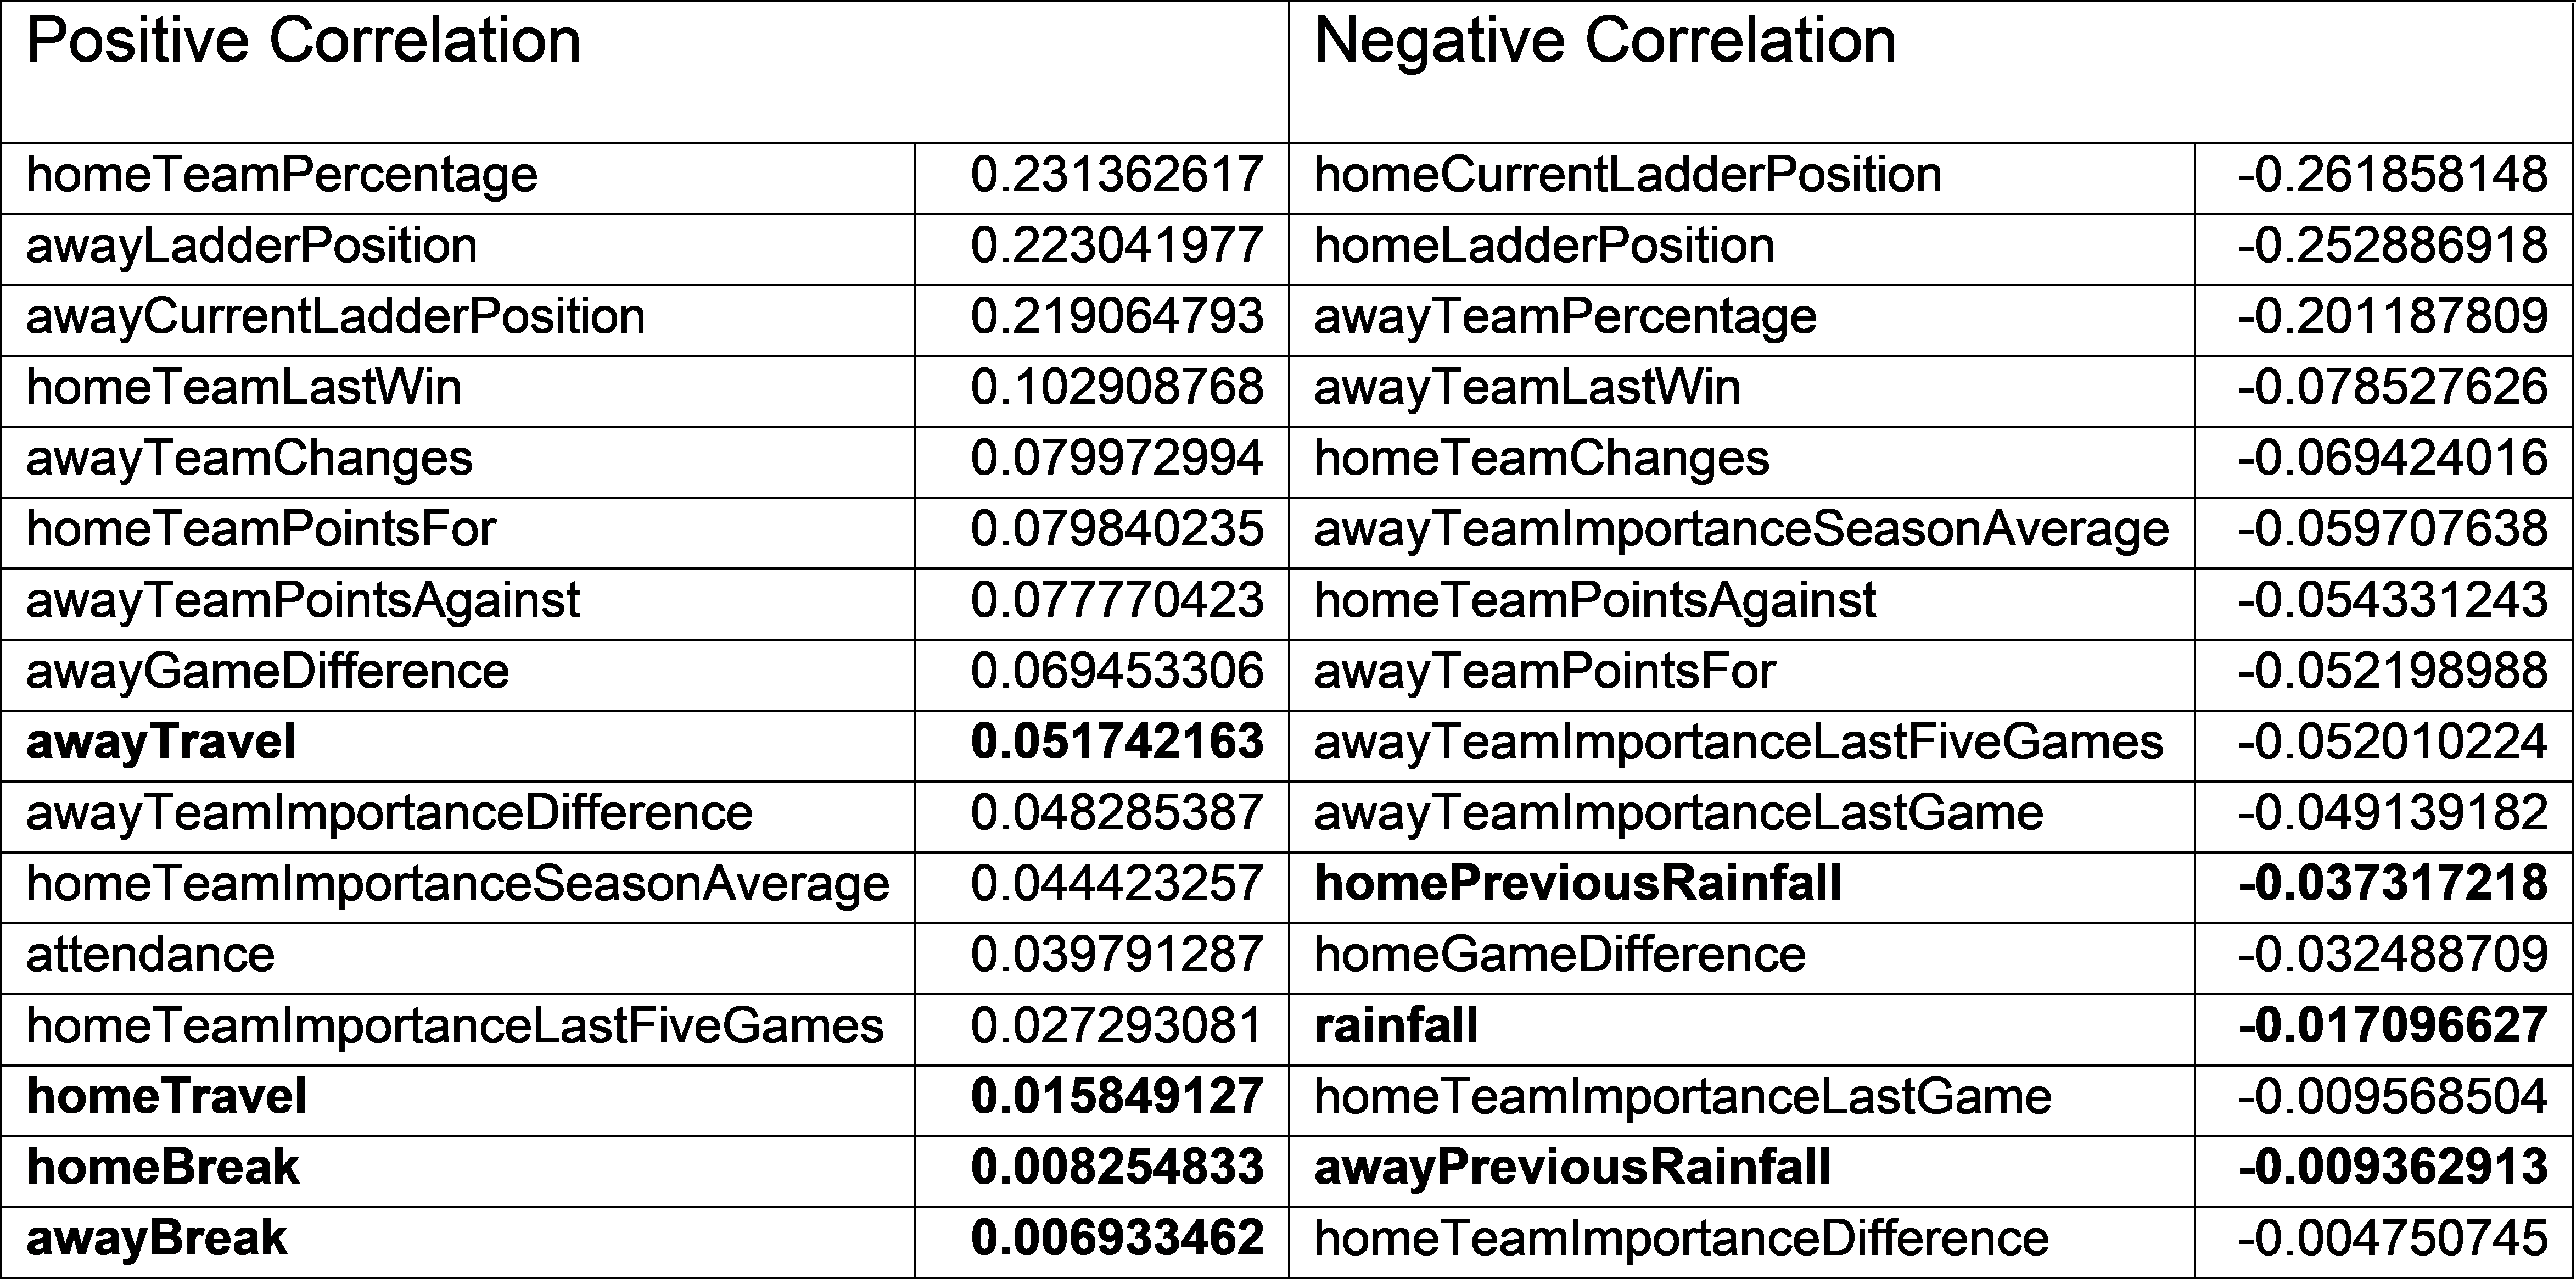
\includegraphics[width=15cm]{media/eda_correlation.png}
	\end{figure}
	The results of the correlation matrix [figure 4.1] can be analysed in two different ways. Analysing the size of the correlation coefficients demonstrates why sports, in this case AFL, can be so difficult to predict, especially in relation to the data set used in the project. As mentioned a correlation of 1 means a perfect positive correlation and -1 the opposite, with 0 meaning no correlation. Only 7 features out of 32 have a coefficient above 0.1 or below -0.1, with a minimum and maximum correlation of -0.26 and 0.23 respectively. As such it is evident that there is a very low correlation between the features and the end results. However ignoring the scale of the coefficient and only looking at the order of the features does produce somewhat expected results. The ladder positions and percentages of each team are the top 3 features for both positive and negative correlation. The reason the ladder positions seem to be in the wrong column is because 1 is the top of the ladder and 18 is the bottom, as such if the teams position is increasing in value they are performing worse.
	
	As for the bold values, which were the features that are generally quoted by experts and casual viewers as having impacts on results, the correlation matrix indicates that these features do have little to no impact on results. Although from their positions an argument can be made that there is a slight home ground advantage as the 'awayTravel' feature ranks relatively high within these features. 
	
	Rainfall having such little impact is also slightly surprising, however this is supported by John Elliot \cite{website:AFL_Weather} in his analysis of the impact of weather conditions in the AFL. What his analysis correctly asserts, that this data set does not take into account and that I did not explore, is that weather is more likely to have a greater impact on individual teams and the favourites leading into the game, as opposed to just the home Team. There is a possibility that a Neural Network would be able to find this connection and possibly the connection with the other highlighted features in question. However I failed to take this into account further into the project, when fitting the data to the Neural Network. To properly assess these features I could have isolated them and used them as input into the Neural Network to assess if the network could find any relationship. But even after isolating the features, it would be very difficult to see the true nature of this relationship due to the black box nature of neural networks.
	
	Another idea explored in the research by Elliot which I did not consider was to classify the weather conditions instead of using the raw numerical rainfall values from the data set. This was also a limitation of the data set, as the data used in Elliot's analysis already provided these categorical values. I did choose to convert the travel features into categorical values however, and this led to similarly poor correlation. This suggests that to better analyse these features in future projects a deeper analysis on each feature should be performed, which would then need to be be translated into data points that can be fit into a prediction model.
	
	\subsection{Feature Engineering Results}
	\begin{figure}
		\caption{Feature Importance Results}
		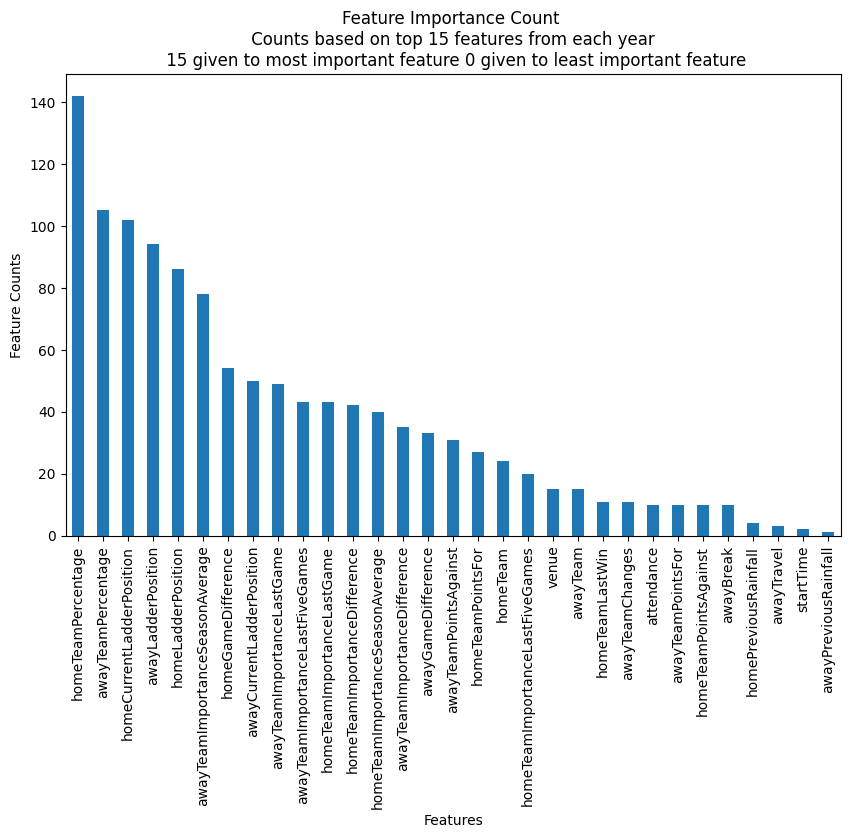
\includegraphics[width=15cm]{media/FeatureImportance.png}
	\end{figure}
	Although some individual features were not as deeply explored, a deeper analysis into the data set as a whole was undertaken in the feature engineering phase. During feature engineering the data from each year was analysed via Random Forest models to discover which features overall had the most impact in the prediction of the outcome of each season. The top 15 features were then extracted into a weighted list, with 15 given to the most important feature and the totals for each feature were tallied, the results can be seen in figure 4.2. Four random forest models were used in this phase, with the first three models being used to extract the features, the final model was then built using only the extracted features. From these features the top 8 pairs were taken for the final data set, these were:
	\begin{table}[h!]
	\caption{Important Features}
	\centering	
	\begin{tabular}{| c | c |}
		\hline
		homeTeamPercentage & awayTeamPercentage\\
		\hline
		homeLadderPosition & awayLadderPosition\\
		\hline
		homeTeamImportanceSeasonAverage & awayTeamImportanceSeasonAverage \\
		\hline
		homeCurrentLadderPosition & awayCurrentLadderPosition \\
		\hline
		homeTeamImportanceLastGame & awayTeamImportanceLastGame \\
		\hline
		homeTeamPointsFor & awayTeamPointsFor \\
		\hline			
		homeTeamImportanceLastFiveGames & awayTeamImportanceLastFiveGames \\
		\hline
		homeTeamPointsAgainst & awayTeamPointsAgainst \\
		\hline		
	\end{tabular}	
	\end{table}

	The top features largely mirrored the top features identified in the correlation matrix, with 5 out of the top six values being present in both sets. Home Team Percentage was the most important feature identified by the feature engineering, it was also the feature with the highest positive correlation in the matrix. 
	
	The biggest change between the two sets were the team importance features. Team importance values were calculated based off of ranking points awarded to each player after a game, and four combinations were calculated for each game. The difference between the previous game and the upcoming game, the average score in each team over the last five games, the average score in each team over the entire season and the average score in the previous game. These values all had very low correlation coefficients, having no apparent correlation to the outcome. However 3 of the 8 features were within the top 10 of the important features and 7 out of 8 in the top 15. 6 of which featured in the final data set.
	
	The main improvement I would make to the feature engineering process is in the generation of the weighted list. When the feature importance is calculated it is also assigned an importance value, which denotes how much impact the feature had on the model. When I build the list I decided to add the weights based on the position of each feature in the importance list rather than its importance weight. At the time I did not consider the impact this might have had on the features chosen for the final data set. Because the difference between the importance values was non linear the sum of the weights most likely have been different to the sum of the positions which I used for this model. It would have been valuable to also calculate the sum of the weights, or even a combination of the position and weights to see if it would have a major impact on the outcome of the feature importance list. However in saying this, a decision would still need to be made as to which features to take, which would have to be a human decision as without further deeper analysis it would be difficult to tell which feature list matched the data model the best.
	
	\subsection{Final Model Results}
	\begin{figure}
		\caption{Final Model Results}
		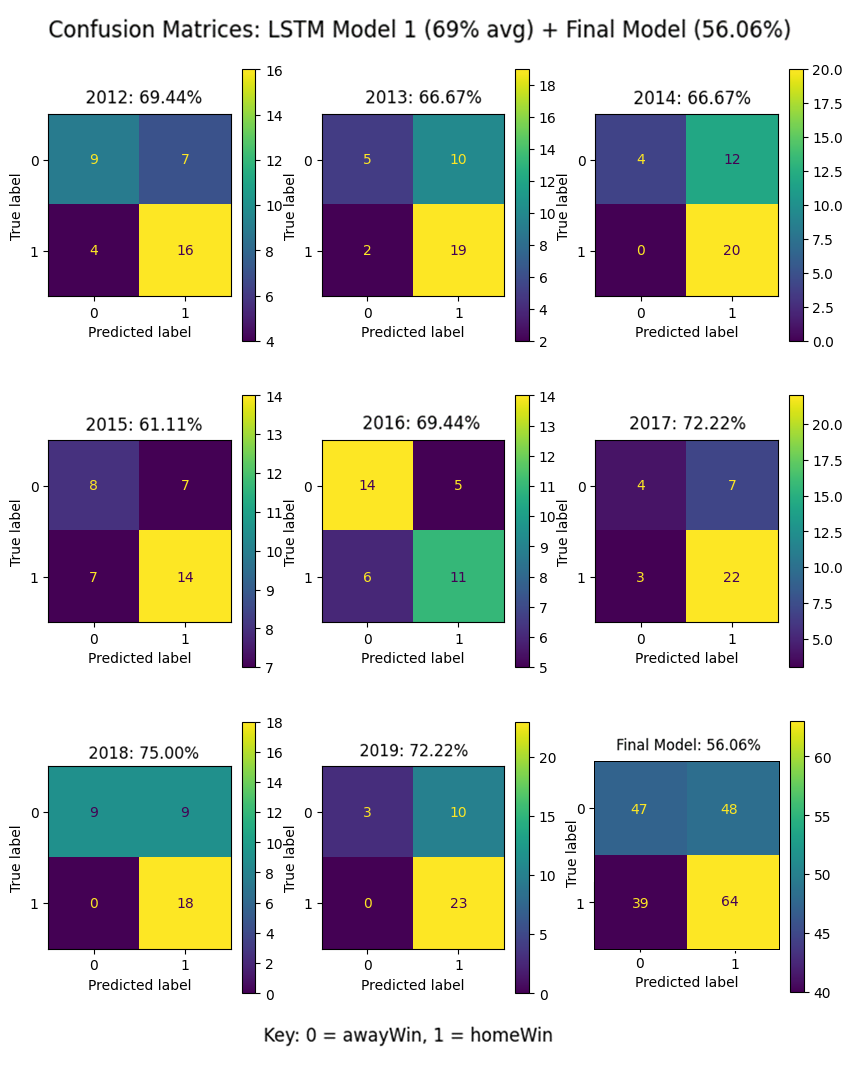
\includegraphics[width=15cm]{media/final_results.png}
	\end{figure}
	The results of the model selection were quite promising. The final model that was selected was able to fit each of the training seasons (2012 - 2019) with an average accuracy of 69\%. With each model individually performing better than the baseline by ~10\%. However one key point that I did not investigate was the baseline for each validation set. The reason I did not explore this was because I did not want to explore any test data too heavily as this can potentially lead to biases in the final model if too much information is extracted from the test data. But in this case I overlooked the fact that data used for the model selection was not the final test data, so I could have performed the simple extraction of the baseline. This would have allowed me to view the homeWin distribution and check that the distribution was still balanced. Most of the models had a bias towards to predicting a homeWin. Interestingly the 2016 model correctly predicted the most away wins, despite having the highest baseline of home wins (59\%).
	
	Unfortunately this accuracy did not translate into the final model trained on the entire data set, as can be seen in the final matrix shown in figure 4.3. Only an accuracy of 56.06\% was achieved, which was much worse than each individual model. Only a 4.5\% improvement was made on the baseline of 51.69\% as opposed to the individual models ~10\% average increase. The key reason for this discrepancy was the differences in the data sets. The individual seasons were trained on only the seasonal data, whereas the final model was trained on data from previous seasons, with in season data only being present in the time window. The only method used to overcome this was adding some contextual data within the data set, which described each teams performance within the season. The impact of this contextual data was supported by the feature engineering, with 14 of the 16 features describing data directly related to a teams performance in the current season. The final 2 features provided historical context of each teams ladder position from the previous season. While some information was able to be learnt from the previous seasons it was important necessary for the model to have data from the current season to improve its accuracy.
	
	\begin{figure}
		\caption{Incremental Round Results}
		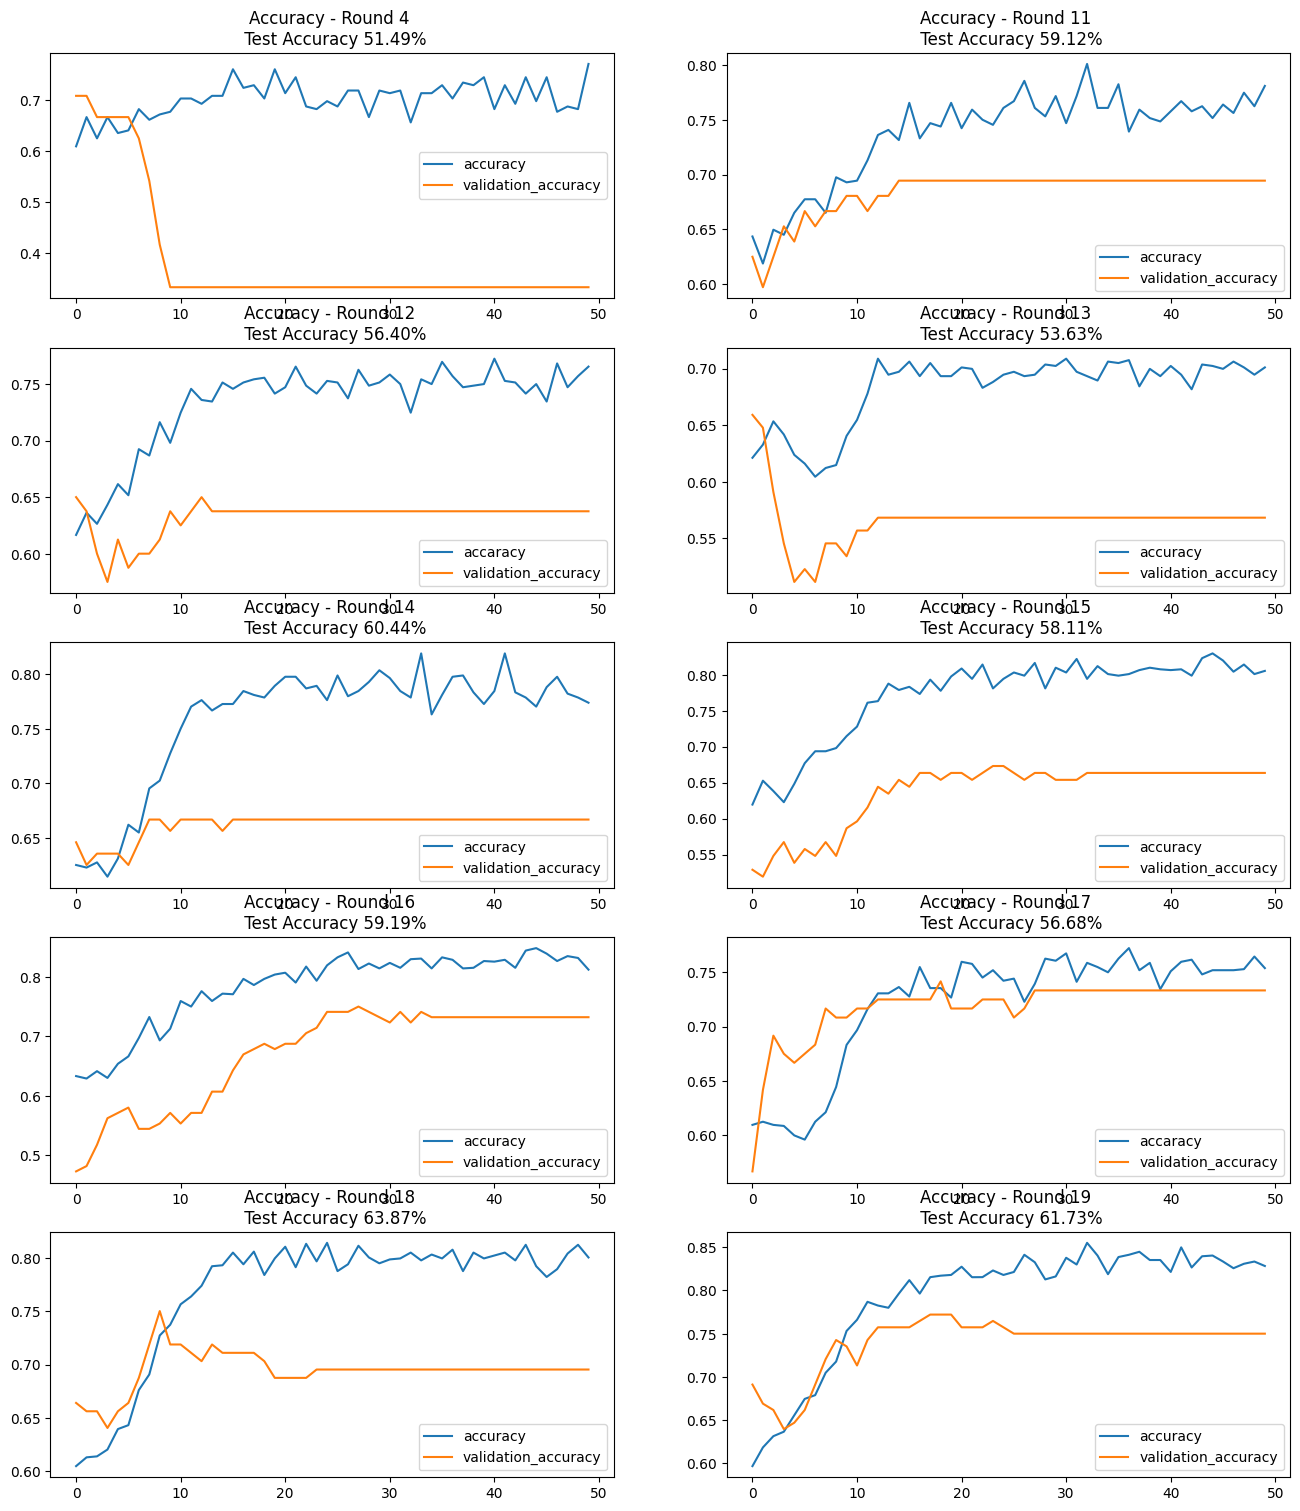
\includegraphics[width=15cm]{media/r4-11-19-acc.png}
	\end{figure}

	This leads to the final research question, how many rounds will the model needs before it becomes reliable. As mentioned in the implementation, I analysed the models performance over multiple variations of each data set. As mentioned in the implementation I originally increased the number of rounds by increments of 3 but due to compromised rounds I decided to analyse each round between round 4 and round 19. 
	The results unfortunately were not very useful from a prediction point of view. Interestingly none of the iterations reached the accuracy from the model selection phase, which further proves that such a high accuracy was the upper limit of the model. The highest accuracy reached in this section was 63.87\% in round 18. 
	Round 11 appears to be where the model begins to reach a more consistent level of prediction, but only to a minor degree, Figure 4.4 displays the accuracy plots for round 4 and of each round from round 11. The mean and standard deviation of the rounds before round 11 are 53.93 and 2.049 respectively, whereas from round 11 they are 58.79 and 3.055. However this includes the three bye rounds two of which have much lower accuracy, removing the three by rounds increases the mean to 59.78 and lowers the standard deviation to 2.598, which is marginally better but still not accurate enough for a reliable prediction model, only being 4\% higher than the baseline.
	
		
	\chapter{Related Works}\label{chap:related_works}
	\subsection{Data Mining}
	Although data mining is not a big subject in sports it is a major influence in many other industries. Data Mining has a very broad use case in both Supervised and Unsupervised learning. Supervised learning is a subcategory of machine learning that deals with data where the input and output is known, as is the case with the data in this paper, it aims to map input data to resulting output data. Supervised learning can be further divided into two categories Classification, where the output is a class or category and Regression where the output is continuous. 
	
	There are many state of the art data mining techniques in both Classification and Regression. There have been some Classification Methods already mentioned in the paper, Decision Trees and Neural. Other widely used algorithms include K Nearest Neighbour (KNN), Support Vector Machines (SVM) and Bayesian Methods \cite{SOTA}. The K Nearest Neighbours attempts to classify a data point based on the class of its Nearest Neighbour points, a SVM is a method that aims to define boundaries to separate a space into classes. Bayesian Methods are more complex it is based upon a method that “combines prior information about a population parameter with new evidence from information contained in a sample to guide the statistical inference process” \cite{website:Britannica}, the basis of the inference is gained through an application of Bayes Theorem \cite{website:Britannica}. The main application of these algorithms is to forecast how a certain input will act based on their characteristics, in the finance industry this can be deciding how likely a customer is to default on their payments based on their previous behaviours, in the medical industry these can be used to predict how likely a patient is to have a certain medical condition.
	
	\subsection{Long Short Term Memory Networks}	
	The state of the art of Long Short Term Memory networks is very centralised around stock market predictions and natural language processing, with some forays into image and video analysis. 
	Time series forecasting, techniques, similar different
	Time Series \cite{10.1145/3453800.3453812}
	
	Stock market predictions, techniques, similarities 
	Indonesia\cite{10.1145/3568231.3568249}
	Bitcoin \cite{10.1145/3546157.3546162}
	Dividend \cite{10.1145/3474880.3474898}
	
	Natural language processing, techniques, similarities, 
	Sentence Embedding \cite{10.1109/TASLP.2016.2520371}
	Spam \cite{10.1145/3234781.3234794}
	
	\subsection{Data Mining in Sports}
	Although there are many state of the art use cases of data mining, they have limited use in the field of sports. As discussed in “Sports Data Mining” by Robert P. Schumaker et al. \cite{SportDM}. This text looks at which data should be collected to properly performing data mining in sports and “how to best make use of it”. It also discusses the issues faced by those entering data mining in sports not only in the initial phases but also the final phases of data mining. One of these difficulties is the relationships between sports organisations and their data, many were unwilling to embrace data mining techniques at the time of the publication of the book. They defined 5 levels of relationships between organisations and the data they produced. Shown below in table 2, taken from Chapter 1, page 2 from the book.
	
	\begin{table}[h!]
		\centering	
		\begin{tabular}{| c | c |}
			\hline
			Level & Relationship\\
			\hline
			One & No relationship \\
			\hline
			Two & Human domain experts make predictions using instinct and gut feeling \\
			\hline
			Three & Human domain experts make predictions using historical data \\
			\hline
			Four & Use of statistics in the decision-making process \\
			\hline
			Five & Use of data mining in the decision-making process  \\
			\hline			
		\end{tabular}
		\caption{\label {tab:Sport Data Relation}Hierarchy of Sport and Sport Data Relationships.}		
	\end{table}
	
	Schumaker claims in the text that at the time of publishing many organisations resided in level 3 or 4 of the hierarchy.  The issue is that there is currently no straightforward way to identify if organisations are using data mining and how they are using it. 
	Another issue highlighted in the text is the inconsistencies and misinterpretations of statistical sports data. As is pointed out in the text many long standing statistics are misleading in modern contexts where we now have a better grasp on these methods and much greater available computing abilities. However, these methods still remain prominent and in use today, as such the book seeks to define new methods to ensure proper algorithms and applications of data analysis and data mining are used. 
	In the book the Data-Information-Knowledge-Wisdom Hierarchy (DIKW) is used to separate techniques and use cases into each of the categories, to identify the best methods and algorithms to be used on each use case. 
		
	Moving into the field of academic papers there are only a handful of resources that explore similar issues to this paper. The most common areas of focus are American Football, Basketball and Baseball. 
	
	Carson Leung and Kyle Joseph, explore a prediction model for American Football in their paper, “Sports Data Mining: Predicting results for the college football” \cite{CollegeFootball}. They employ an interesting dropout technique for their prediction model, in which they do not explore the results of the two teams that will be predicted, instead focusing on “a set of teams that are the most similar to each of the competing teams” \cite{CollegeFootball}, [page 716]. Similarly, they identify statistics on which the final model will be based, but only 4 instead of the larger set as in the model in this paper.
	
	On the more analytical side is the paper “Sports analytics— Evaluation of basketball players and team” by Vangelis Sarlis and corresponding author Christos Tjortjis. This paper looks at and “evaluates the existing performance analytics used in Europe and NBA (in USA) basketball” \cite{Basketball}. They identify two metric types, Player and Team, and four criteria groups; Key Performance Indicators (KPIs), Defensive criteria, Offensive Criteria and Overall Performance Criteria, as well as outlining a Comparison Matrix and Data Mining Techniques used in sports analysis. They also explore if they can optimise existing performance analysis metrics that are used in basketball. 
	
	An overall review of the current techniques used in sports prediction (as of 2013) is given in the paper “A review of Data Mining Techniques for Result Prediction in Sports”, M. Haghighat et al., \cite{ResearchGate}. 6 Methods are analysed in the resource of which two, Artificial Neural Networks and Decision Trees are used in this paper. Bayesian Method, Logistic Regression, Support Vector Machines and Fuzzy Methods are the other methods that are analysed. Since nearly 10 years have passed since this resource was published, there has been many improvements to the models that are used in this paper, specifically in the field of Neural Networks. 
	
	A more limited set of comprehensive work has been completed regarding Data Science and Australian Football. In 2008 McCabe and Travathan briefly explored the usability of neural networks in predicting the outcomes of sports in their conference paper “Artificial Intelligence in Sports Prediction” \cite{AFL_1}. Here they reached an average accuracy of around 65 percent using 11 performance metrics. This model did not only focus on AFL, it also aimed at predicting Rugby League, Rugby Union and Soccer, as such the features used were not specific to any of the predicted sports. The model in this paper aims to be more specific to features occurring in AFL. 
	
	H. Jelenik et al in their article “Using meta-regression data mining to improve predictions of performance based on heart rate dynamics for Australian football” \cite{AFL_2}, follows a similar scientific method to that which is used in this paper, utilising Random Forest algorithms to extract key features from the dataset. However the type of data differs greatly, this article features gps data and medical data with the predictions being more focused on individual player performance as opposed to team performance prediction. M. Aarons et al also utilised GPS data in their article on “The effect of team formation on defensive performance in Australian \cite{AFL_3}, which analysed a team’s defensive positioning and the effect it had on defensive performance, similarly to this paper decision tree analysis was also utilised in the article, however the majority of the methods and data differed. These both used minimal similar decision tree and random forest techniques in their analysis but the data set and overall prediction scopes differed from what was used in this paper. 
	
	Sports ML \cite{BUNKER201927}
	
	Human Activity Modelling \cite{10.1145/3316782.3322781}
	
	\newpage
	\chapter{Summary}\label{chap:summary}
	\section{Summary}
	Overall this paper aimed to explore and understanding the use of Data Mining in Professional Sports, specifically the Australian Football League. It aimed to build upon methods already being used in sports data mining and to combine them with existing methods being utilised in other fields of data mining and to explore the following research questions:
	\begin{enumerate}
		\item[] Can data mining be used to find key features and patterns and explain results in professional sports?
		
		\item[]Can these extracted trends and features be used to create a reliable prediction model?
		
		\item[] How can the results be utilised in the sporting industry?
		
		\item[] If the model can reliably predict outcomes, how many rounds will the model need before it becomes reliable?
	\end{enumerate}
	
	The results of the paper were varied, many improvements could have been made to the processes used in the project. With more time and resources the quality of the data could have been greatly improved as well as utilising different techniques and methods when defining the data set. 
	Continuous vs discrete data. A greater use of discrete data could have been used to increase the expressiveness of the data. The majority of the final data set was continuous.
	Data complexity \cite{ML_Soccer} warn that adding complexity to data does not always lead to better results in sports predictions. There are many factors that can influence the outcome of a game which are not always indicative of a teams strength these can be affected by random chance or human factors and therefore are had to quantify and analyse in a model. Although I believe adding additional complexity to the data in this case could have been useful, specifically in the case of team travel and home ground advantages. In the model I only looked at basic factors in this regard of, where the game was being played and categorised how far each team needed to travel to reach the destination venue. TheAFLLAb \cite{website:AFL_HG} investigates this topic in much greater depth analysing an additional 5 features. 
	
	A major change I would make in subsequent work on this topic would be to change the neural network used to create the prediction model. Long Short Term Memory Networks are designed to handle time series and sequential data. As sport seasons are in general also sequential by nature I believed that the data set could be adapted in a manner that would be able to be fit to the LSTM model. However there were some problems with the data mapping which I did not initially take into consideration when I began the project. Although the data was sequential, LSTM models are also built to handle data in time steps which lead into each other. The issue with sports data is that every game is independent and thus the weights from the game
	\newpage
	\bibliography{refs_thesis}
	\bibliographystyle{ieeetr}
	
\end{document}


\section{Adding images}
Adding a simple image is easy. Adding complex images is also easy. What is a complex image anyway? 
\begin{figure}[h]
	\centering
	
\includegraphics[width=1.0\textwidth]{imclogo.png}
	\caption{IMC Logo}
	\label{fig:logo}
\end{figure}




